\newpage
\section{Diskussion}
\label{sec:Diskussion}

Die Werte, die in \autoref{sec:Auswertung} berechnet wurden, sollen im folgenden auf ihre Genauigkeit untersucht und diskutiert werden.

\subsection{Diskussion der Kennlinienschar}
\label{subsec:DiskKenn}
Zu der Kennlinienschar ist anzumerken, dass die Möglichkeit besteht, dass die Sättigungsströme nicht bei jeder Messung vollständig erreicht wurde.
Zwar flachen die Kennlinien für die ersten drei Heizleistungen($\SI{5,7}{\watt},\ \SI{7,0}{\watt},\ \SI{8,1}{\watt}$) sehr schnell ab, allerdings 
sind aus \autoref{fig:plot1} nicht die Sättigungsströme für die Heizleistungen von $\SI{10,35}{\watt}$ und $\SI{13,75}{\watt}$ abzulesen. Es wurde deshalb eine
Regression dritten Grades angelegt, bei der festgestellt wurde, dass der Sättigungsstrom für $\SI{10,35}{\watt}$ doch aus \autoref{fig:plot1} abzulesen ist.
Die Werte davon sind in \autoref{tab:saettis} eingetragen.

\subsection{Diskussion des Gültigkeitsbereich des Langmuir-Schotky'schen Raumladungsgesetzes}
\label{subsec:DiskLangmuir}
Bei der Auswertung des Langmuir-Schotky'schen Raumladungsgesetzes ergab sich eine Steigung der linearen Regression von $m = 1,437 \pm 0,0146$, was einer
Abweichung um $(4.2 \pm 1.0)\%$ vom Theoriewert $m = 1.5$ entspricht.
Die Abweichung ist damit als so gering einzuschätzen, dass zu sagen ist die Theorie bestätigt zu haben. \newline
Grund für diese Abweichungen können sein, dass die Geräte nicht richtig eingestellt wurden oder die Werte von dem analogen Milliamperemeter nicht sorgfältig genug abgelesen wurden. Ein digitales Messgerät oder mehr Messwerte können
diesen beiden Fehlern entgegenwirken.

\subsection{Diskussion des Anlaufstromgebietes}
\label{subsec:diskAnlauf}
Bei der Untersuchung des Anlaufstromgebietes musste am analogen Milliamperemeter mehrmals der Messwertebereich geändert werden. Da bei jedem umstellen gewisse Unsicherhieten auftauchen,
ist der stufenförmige Verlauf der Messwerte in \autoref{fig:plot2} zu erklären. Dieser Fehler kann verringert werden, indem mehr Messwerte genommen werden oder ein digitales
Amperemeter verwendet wird, dessen Messwerteberich den vollen Aufnahmebereich abdeckt.

\subsection{Diskussion der Kathodentemperaturen und Austrittsarbeiten}
\label{subsec:diskTemps}

In \autoref{subsec:kathodenTempSchar} und \autoref{subsec:richard} ergaben sich die in \autoref{tab:diskussi} eingetragenen Werte für die Kathodentemperaturen und Austrittsarbeiten.
Die Kathodentemperatur, die mithilfe des Anlaufstromgebietes bestimmt wurde, beträgt $T_1 = \SI{2865,095 \pm 343,460}{\kelvin}$.
\begin{table}[H]
    \caption{Kathodentemperaturen $P_{\text H}$ und Austrittsarbeiten $\phi$ mit den jeweiligen Heizleistungen und Sättigungsströmen.}
    \label{tab:diskussi}
    \centering
    \begin{tabular}{c c c c}
        \toprule
        $P_{\text H} \,/\, \si{\watt}$ & $I_{\text S} \,/\, \si{\milli\ampere}$ & $T \,/\, \si{\kelvin}$ & $\phi \,/\, \si{\eV}$\\
        \midrule
        $13,75$ & $3,7 \pm 0,7$   & $2229,3641$ & $4,740 \pm 0,035$ \\
        $10,35$ & $1,14 \pm 0,12$ & $2073,9679$ & $4,593 \pm 0,018$ \\
        $8,1$   & $0,284$         & $1936,8526$ & $4,499$ \\
        $7,0$   & $0,11$          & $1857,6287$ & $4,453$ \\
        $5,7$   & $0,047$         & $1748,6121$ & $4,302$ \\
        \bottomrule
      \end{tabular}
  \end{table}

  \noindent
Die ausgerechneten Werte der Kathodentemperaturen können mit keinen Theoriewerten verglichen werden. Allerdings können die Temperaturen, die sich
bei einer Heizleistung von $\SI{13,75}{\watt}$ ergeben haben, miteinander verglichen werden.
Es folgt eine Abweichung von $\upDelta T = (29 \pm 15)\%$. Das kann mit den Gründen aus \autoref{subsec:diskAnlauf} erklärt werden.
Die Abweichung des Mittelwertes der Austrittsarbeit $\overline\phi = \SI{4,517 \pm 0,008}{\eV}$ vom Literaturwert $\phi_{\text Lit} = \SI{4,55}{\eV}$
beträgt $(0.29 \pm 0.15)\%$.
Die Abweichung ist sehr gering und die Theorie wurde damit verifiziert.

\printbibliography{}

\section*{Anhang}
\label{sec:anhang}

\begin{figure}[H]
    \centering
    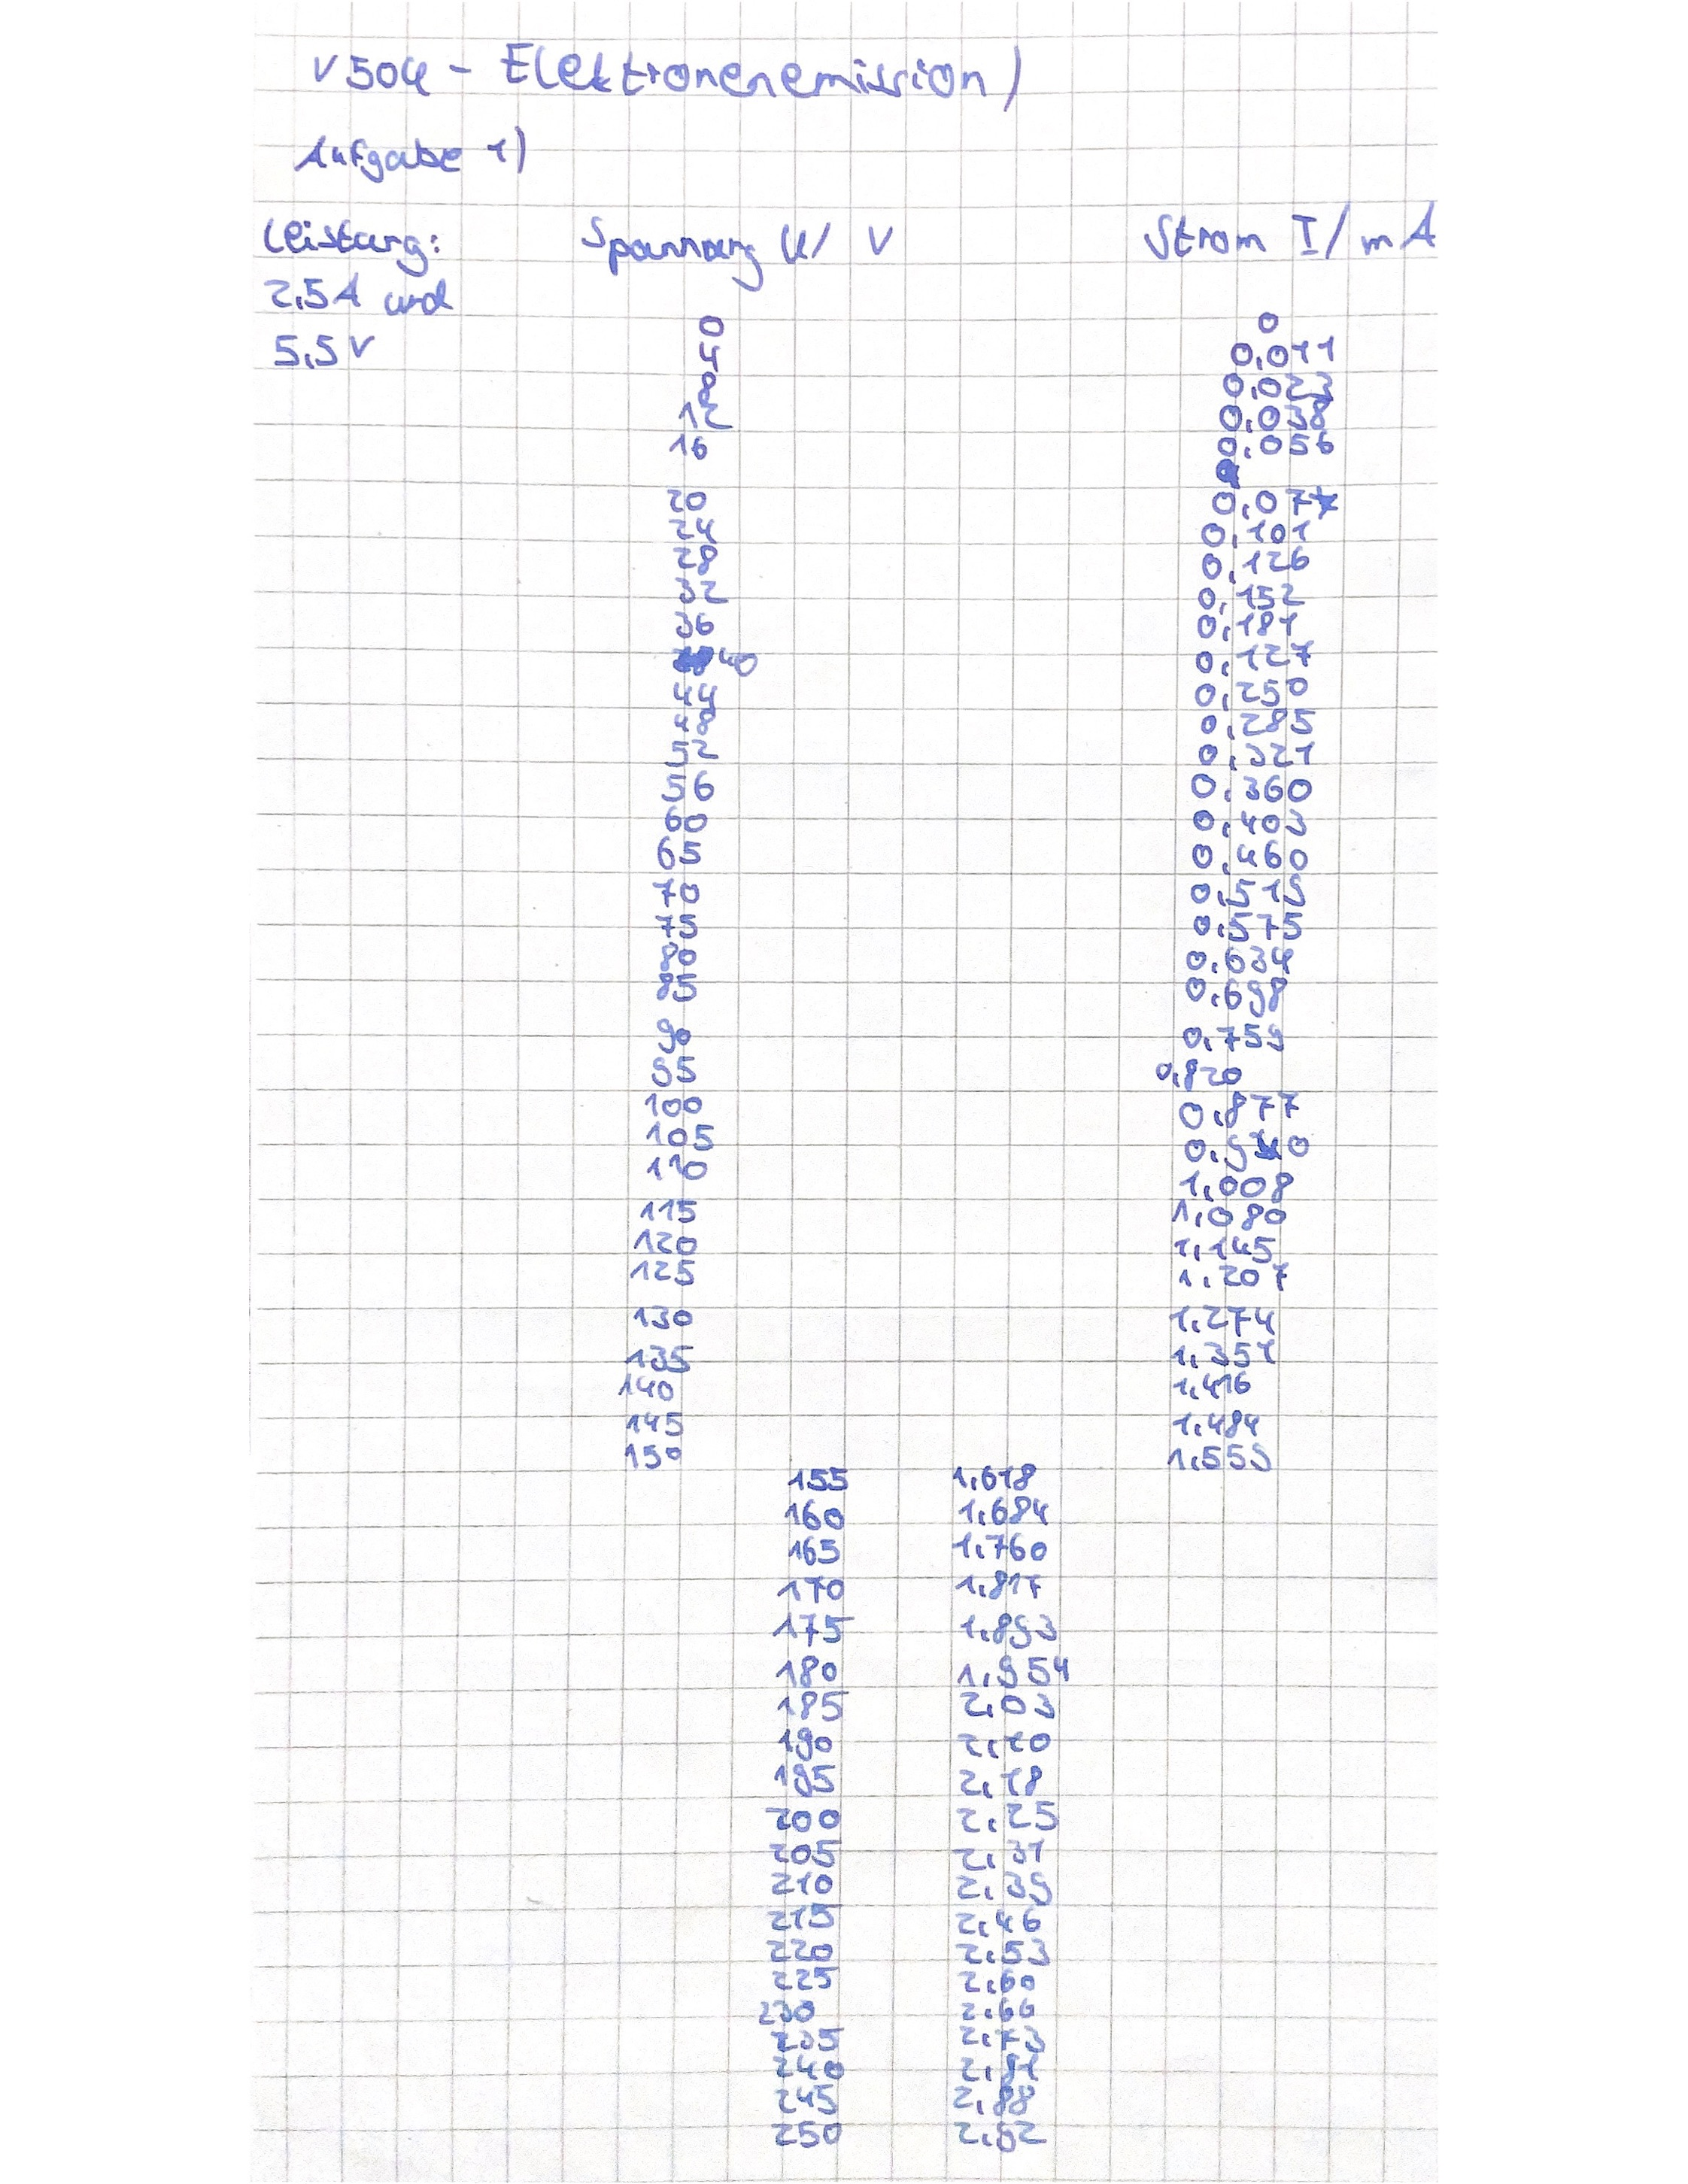
\includegraphics[width=0.7\textwidth]{data/origDaten1.jpg}
    \caption{Originale Messdaten.}
    \label{fig:origDaten1}
\end{figure}

\begin{figure}[H]
    \centering
    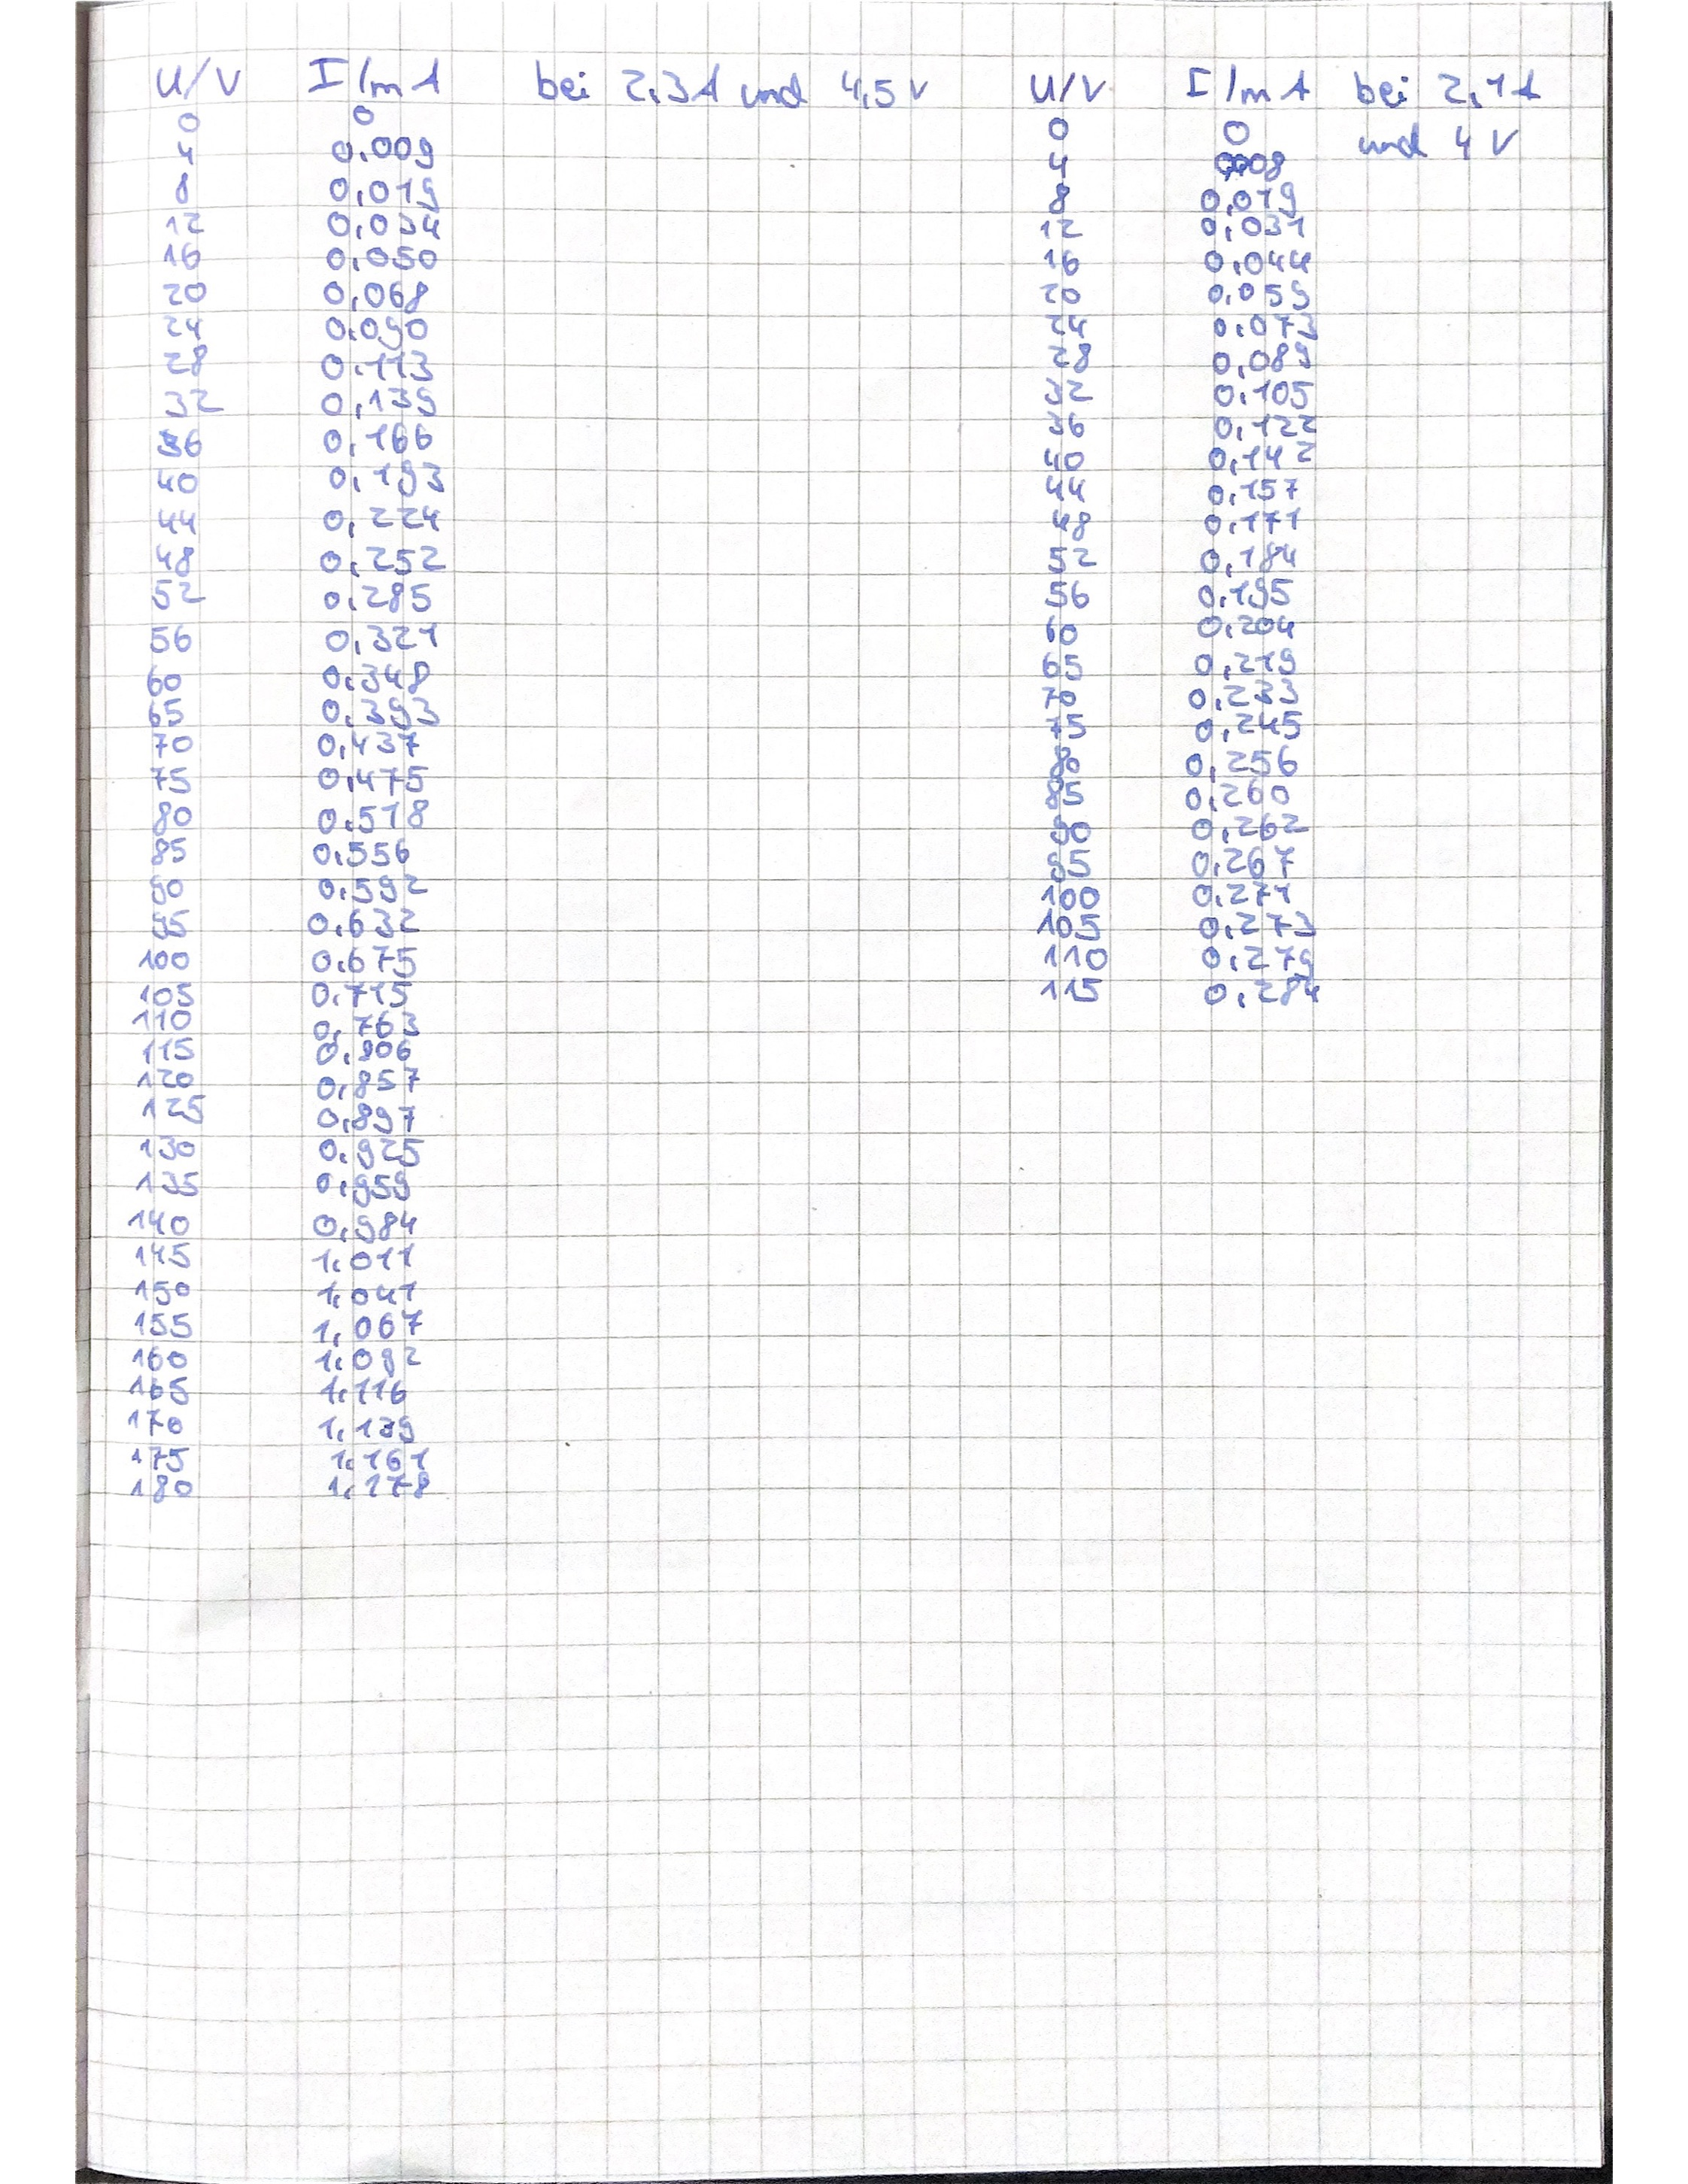
\includegraphics[width=0.7\textwidth]{data/origDaten2.jpg}
    \caption{Originale Messdaten.}
    \label{fig:origDaten2}
\end{figure}

\begin{figure}[H]
    \centering
    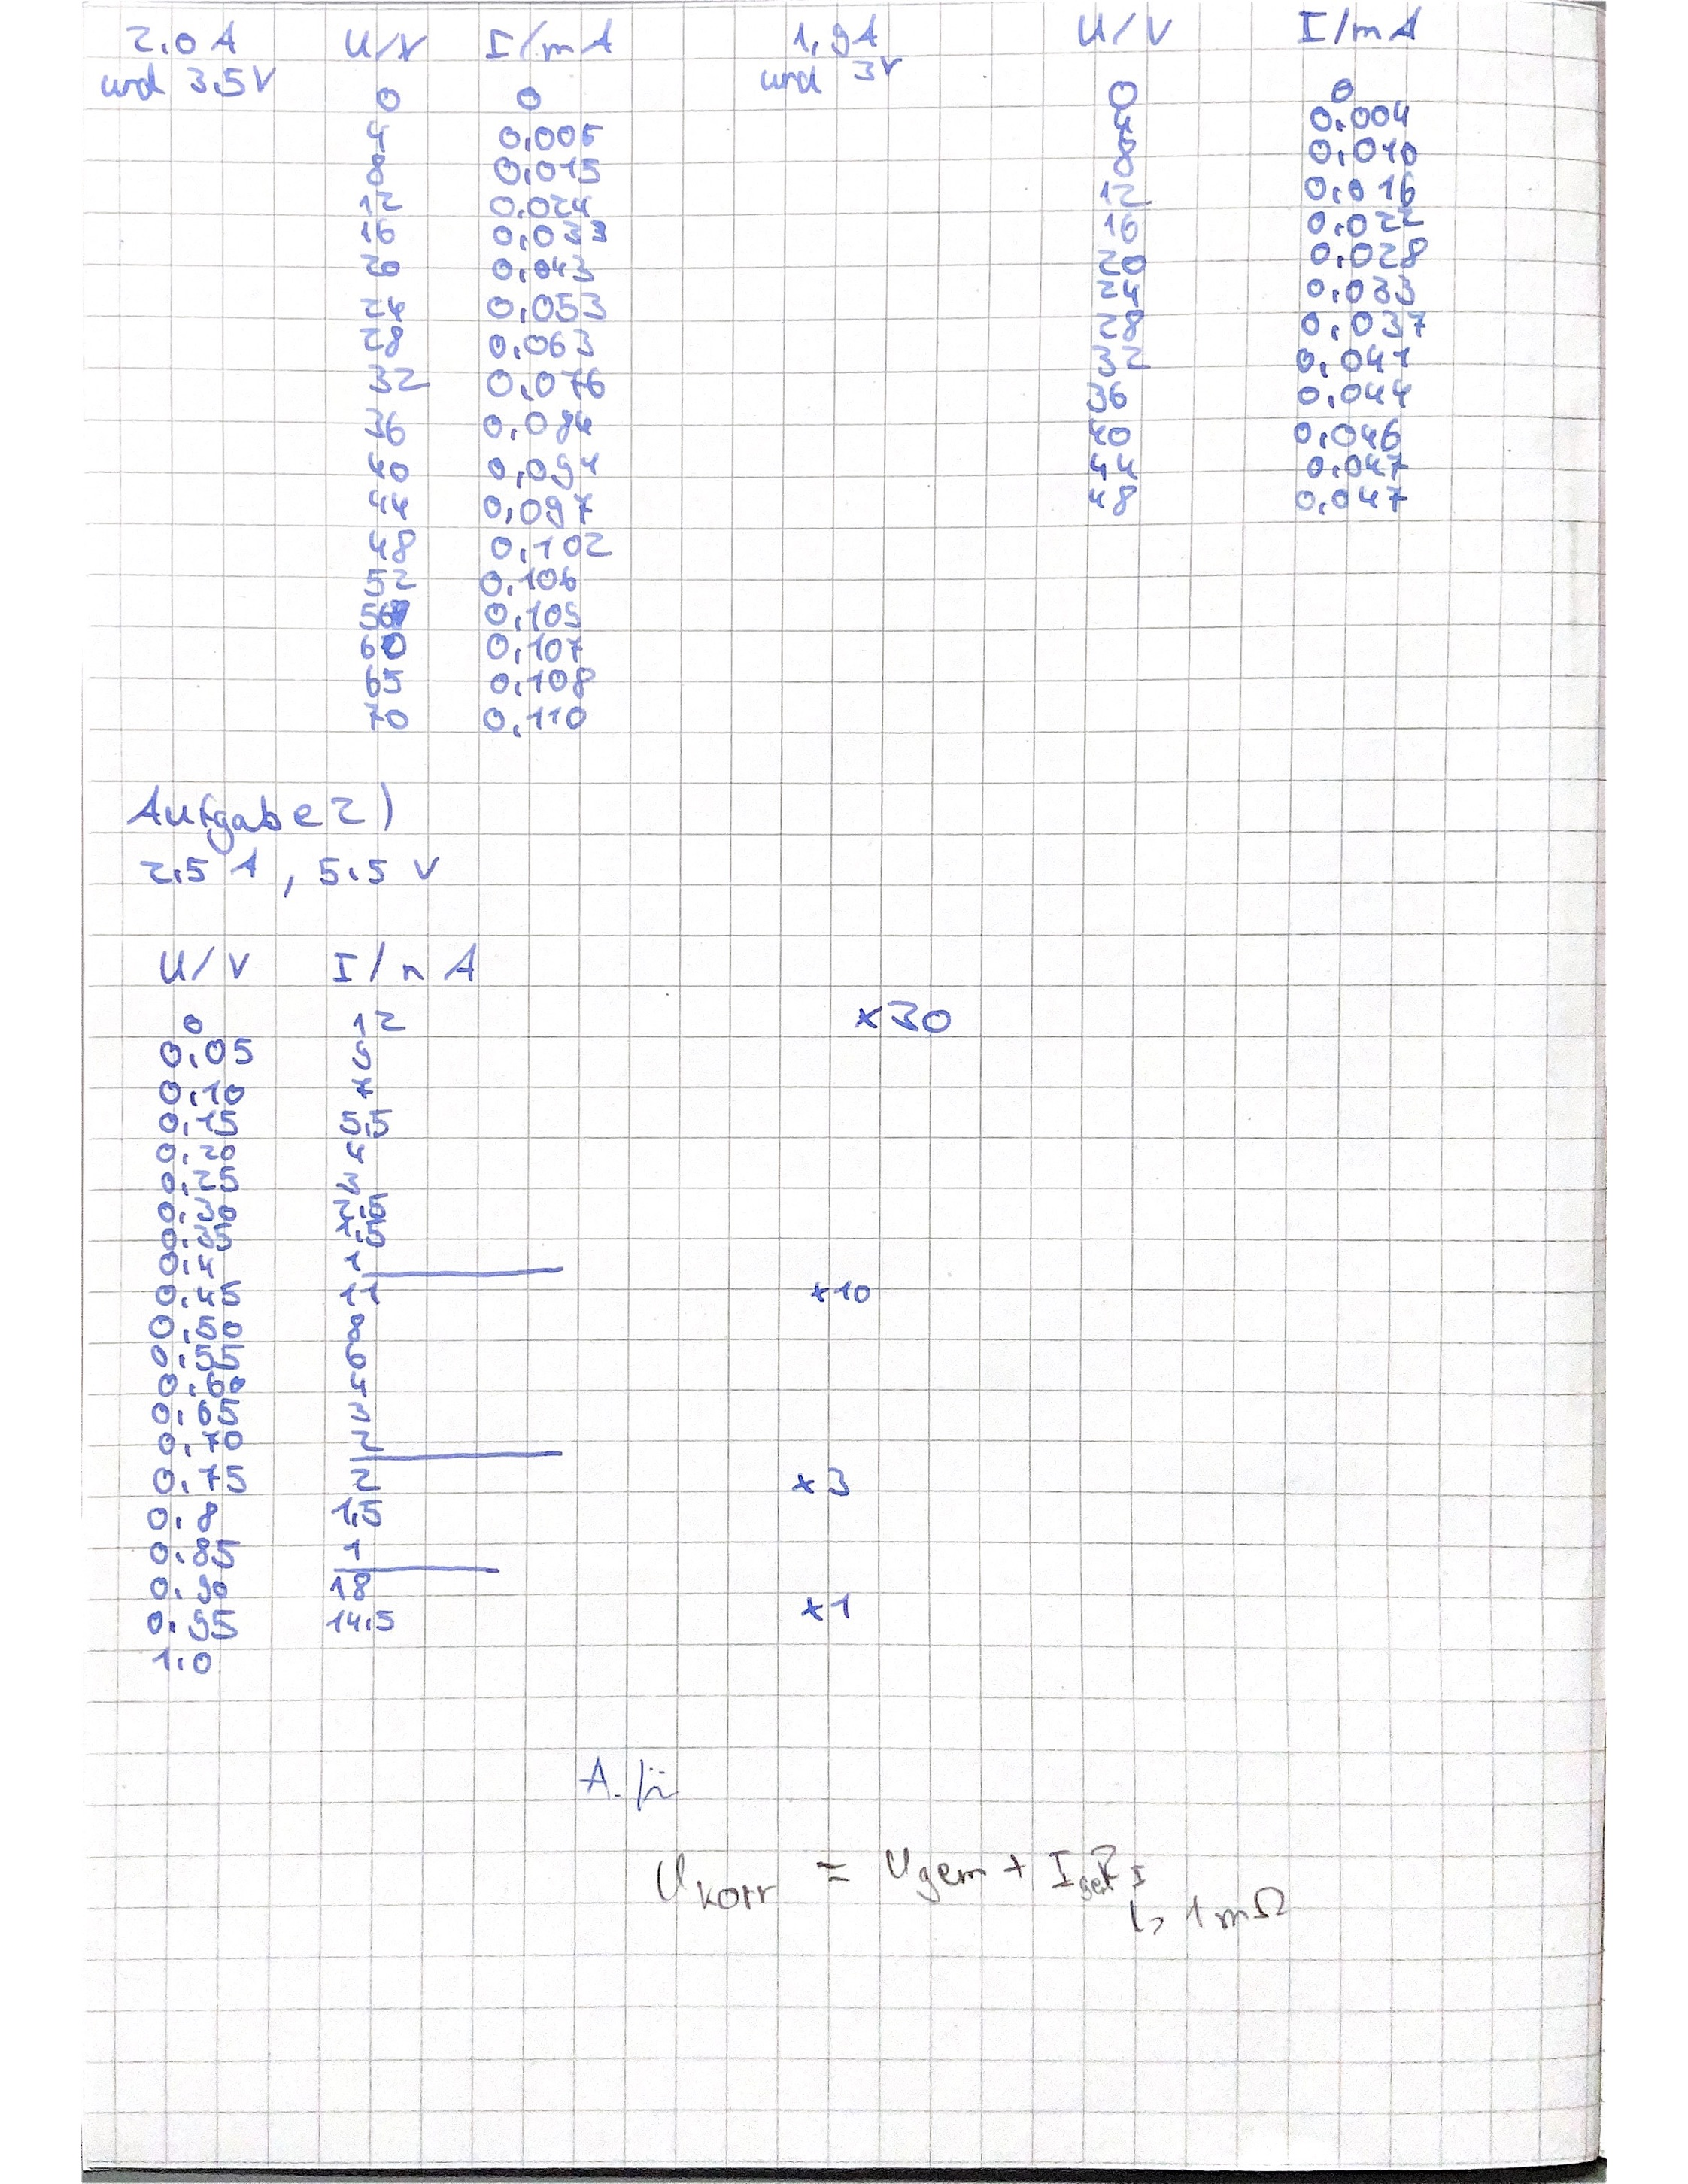
\includegraphics[width=0.7\textwidth]{data/origDaten3.jpg}
    \caption{Originale Messdaten.}
    \label{fig:origDaten3}
\end{figure}